\documentclass{report}

\input{../LatexTemp/preamble}
\input{../LatexTemp/macros}
\input{../LatexTemp/letterfonts}
\usepackage{xcolor}
\usepackage{tikz-qtree}
\usepackage{graphicx}

% Tikz libraries %
\usetikzlibrary{automata, positioning, arrows}

% Impostazioni Tikz %
\tikzset{
->, % makes the edges directed
>=stealth, % makes the arrow heads bold
node distance=3cm, % specifies the minimum distance between two nodes. Change if necessary.
every state/.style={thick, fill=gray!10}, % sets the properties for each ’state’ node
initial text=$start$, % sets the text that appears on the start arrow
}

% Tikz shapes (manca initial, state e accept) %
\tikzstyle{process} = [rectangle, minimum width=3cm, minimum height=1cm, text centered, draw=black, fill=orange!30]
\tikzstyle{decision} = [diamond, minimum width=3cm, minimum height=1cm, text centered, draw=black, fill=green!30]
\tikzstyle{arrow} = [thick,->,>=stealth]

\title{\Huge{Linguaggi di programmazione}\\Appunti}
\author{\huge{GioLaPalma}}
\date{}
\pagenumbering{gobble}

\graphicspath{{paginette/img/}}

\begin{document}

\maketitle
\newpage% or \cleardoublepage
% \pdfbookmark[<level>]{<title>}{<dest>}
\pdfbookmark[section]{\contentsname}{toc}

\tableofcontents

\pagebreak

\include{paginette/introduzione_ai_linguaggi_normali_grammatiche}
\include{paginette/struttura_di_un_compilatore_sematica_statica_semantica_dinamica}
\include{paginette/linguaggi_liberi_deterministici}
\include{paginette/top_down_parser}
\chapter{Bottom up parser}

Il \textbf{parser bottom up} è un tipo di analizzatore sintattico che che costruisce l'albero di derivazione partendo dalle foglie, viene anche detto \textbf{Shift-Reduce} in quanto possiede due operazioni fondamentali:
\begin{itemize}
    \item \texttt{Shift}: un simbolo terminale viene spostato dall'input alla pila 
    \item \texttt{Reduce}: una serie di simboli (terminali e non terminali) sulla cima della pila corrisponde al "reverse" di una parte destra di una produzione, ovvero:
    \[
        A\to\alpha \in R - \alpha^R \text{ sulla pila}
    \]
    La stringa $\alpha^T$ viene rimossa dalla pila e sostituita con $A$, quindi $\alpha$ viene ridotta ad $A$
\end{itemize}

Inoltre è un \textbf{parser LR} perché:
\begin{itemize}
    \item L: leggo da sx a dx
    \item R: derivazione rightmost
\end{itemize}
 
Possono essere di diversi tipi

\section{Parser shift-reduce nondeterministico}
\begin{algorithm}
    \caption{Parser shift-reduce nondeterministico}
    \KwIn{Una grammatica libera $G$ con simbolo iniziale $S$ e una stringa $w\in T^*$}
    \KwOut{Una stringa $w\in T^*$}

    Inizializziamo la pila a $\$$\;
    Inizializziamo l'input con $w\$$\;
    usaimo il $PDA$ seguente per trovare la derivazione per $w\$$:
    \[
        M=(T, \{q\},\underbracket{T\cup NT \cup \{\$\}}_{\Gamma: \text{ovvero i simboli sulla pila}}, \delta, \varnothing)
    \]
    Dove:
    \begin{enumerate}
        \item $(q,aX)\in \delta (q,a,X)\forall A\in T\forall X\Gamma\quad \text{SHIFT}$
        \item $(q,A)\in\delta(q,\epsilon, \alpha^R)$ se $A\in \alpha\in R\quad \text{REDUCE}$
        \item $(q,\epsilon)\in \delta(q,\$,S\$)\quad \text{accept}$
    \end{enumerate}\;
    ogni volta che facciamo "reduce", forniamo in output la produzione usata\;
    alla fine, $S\$$ sulla pila, con $\$$ in input $\implies$ accettiamo\;
\end{algorithm}

\nt{
    generalizzazione della def. di $PDA$ dove non si consuma solo il top della pila, ma una serie di caratteri contigui a caminciare dal top
}

\esempio{
    Sia la seguente grammatica
    \[
        \begin{array}{l}
            E\to T\mid T+E \mid T-E\\
            T\to A\mid A*T\\
            A\to a\mid b\mid (E)
        \end{array}
    \]
    \[
        \begin{array}{|c|l|l|l|l|}
        \hline
        \textbf{N.} & \textbf{Pila} & \textbf{Input} & \textbf{Azione} & \textbf{Output} \\ \hline
        1  & \$                  & a+b*b\$              & Shift         &                 \\ \hline
        2  & \$a                & +b*b\$               & Reduce        & A \to a         \\ \hline
        3  & \$A                & +b*b\$               & Reduce        & T \to A         \\ \hline
        4  & \$T                & +b*b\$               & Shift         &                 \\ \hline
        5  & \$T+               & b*b\$                & Shift         &                 \\ \hline
        6  & \$T+b              & *b\$                 & Reduce        & A \to b         \\ \hline
        7  & \$T+A              & *b\$                 & Shift         &                 \\ \hline
        8  & \$T+A*             & b\$                  & Shift         &                 \\ \hline
        9  & \$T+A*b            & \$                   & Reduce        & A \to b         \\ \hline
        10 & \$T+A*B            & \$                   & Reduce        & T \to A * T     \\ \hline
        11 & \$T+A*T            & \$                   & Reduce        & E \to T + T     \\ \hline
        12 & \$E                & \$                   & Reduce        & E \to T + T     \\ \hline
        13 & \$E                & \$                   & Accept        &                 \\ \hline
        \end{array}
    \]

    Si ha che:
    \[
        E\implies T+E\implies T+T \implies T + A* T \implies T+A*A \implies T + A * b \implies T + b * b \implies A + b*b  \implies a + b*b
    \]

    Il cui albero è:
    \begin{center}
        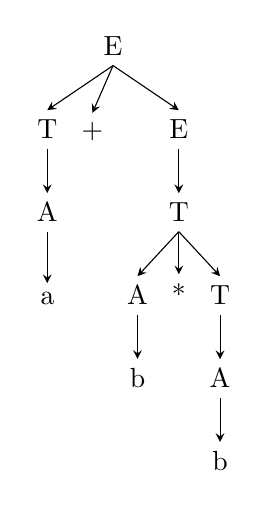
\begin{tikzpicture}
            \Tree [
                .E
                [
                    .T
                    [
                        .A
                        [
                            .a
                        ]
                    ]
                ]
                [
                    .+
                ]
                [
                    .E
                    [
                        .T
                        [
                            .A
                            [
                                .b
                            ]
                        ]
                        [
                            .*
                        ]
                        [
                            .T
                            [
                                .A
                                [
                                    .b
                                ]
                            ]
                        ]
                    ]
                ]
            ]
        \end{tikzpicture}
    \end{center}
    
    Le cui proprietà sono:
    \begin{center}
        \item Costruzione dell'albero di derivazione \texttt{bottom-up}    
        \item Derivazione canonica a destra a rovescio
        \item forte non-determinismo:
        \begin{itemize}
            \item \textbf{conflitti shift-reduce}:
            \begin{itemize}
                \item $\$a \quad +b*b\$ \quad \text{shift}$
                \item $\$ a+ \quad b*b \$$
            \end{itemize}
            \item \textbf{Conflitti reduce-reduce}
            \begin{itemize}
                \item $\$T+A*T\quad\$$ reduce $E\to T$
                \item $\$T+A*E\quad\$$
            \end{itemize}
        \end{itemize}
    \end{center}
}

\nt{Si noti quindi che questo tipo parser genera moltissimi confilitti, in diverse sistuazioni era appunto possibile scegliere strade che non portano a riconoscere la stringa. F}

Per "risolvere" tale nondeterminismo occorre fornire al PDA una tabella parsing (struttura di controllo) che "aiuti" a scegliere l'azione giusta, ed è grazie all'uso di questa che nascono i cosiddetti \textbf{parser LR}

\section{Parser LR}


zio pera
\end{document}
